\documentclass{article}
\usepackage[margin=1in]{geometry}
\usepackage{amsmath,amssymb,booktabs,graphicx,hyperref}
\usepackage{tikz}
\usetikzlibrary{arrows.meta,positioning}
\title{The Human Data Budget: Joint Time-and-Mode Allocation in Recursive Training}
\author{Anonymous August 2026 Project Draft}
\date{}

% Result numbers quoted in section prose are defined here and generated from immutable
% chain artifacts by scripts/generate_pilot_outputs.py. Sections cite macros rather than
% literals so prose cannot drift from the run, which is what
% tests/analysis/test_generated_outputs.py enforces.
% AUTO-GENERATED by scripts/generate_pilot_outputs.py. DO NOT EDIT VALUES BY HAND.
% Every result number quoted in paper/sections/ is defined here and computed
% from chain_result.json artifacts, so prose cannot drift from the run.
% run: primary_pilot_2026-08-18
\newcommand{\PilotCVHigh}{1.08}
\newcommand{\PilotCVLow}{0.41}
\newcommand{\PilotCeiling}{750{,}000}
\newcommand{\PilotChains}{25}
\newcommand{\PilotHorizon}{10}
\newcommand{\PilotJointSelHigh}{0.019}
\newcommand{\PilotJointSelLow}{-0.003}
\newcommand{\PilotJointSelPct}{0.36}
\newcommand{\PilotJointShortfall}{75{,}807}
\newcommand{\PilotJointShortfallPct}{10.1}
\newcommand{\PilotJointSpend}{674{,}193}
\newcommand{\PilotMatchedHigh}{749{,}995}
\newcommand{\PilotMatchedLow}{749{,}709}
\newcommand{\PilotMatchedSpreadPct}{0.038}
\newcommand{\PilotPairedSD}{0.0088}
\newcommand{\PilotRandNoneHigh}{-0.096}
\newcommand{\PilotRandNoneLow}{-0.129}
\newcommand{\PilotRandNonePct}{4.28}
\newcommand{\PilotSchedRandHigh}{0.058}
\newcommand{\PilotSchedRandLow}{-0.016}
\newcommand{\PilotSchedRandPct}{0.84}
\newcommand{\PilotSeeds}{5}
\newcommand{\PilotSelRandHigh}{-0.188}
\newcommand{\PilotSelRandLow}{-0.235}
\newcommand{\PilotSelRandPct}{8.37}
\newcommand{\PilotThresholdPct}{2}
\newcommand{\PilotThresholdUnits}{0.0463}
\newcommand{\PilotWallHours}{6.7}


\begin{document}
\maketitle
\begin{abstract}
Recursive training on model-generated data degrades a language model, and retaining
human-origin data in the mixture substantially reduces that degradation. This leaves a
question open: under a \emph{fixed lifetime budget} of human-origin optimizer tokens, when
during recursive training should those tokens be spent, and which under-covered modes of a
human reference distribution should they target? We predefine four budget-matched treatment
families --- random rescue, schedule-only, selection-only, and a joint time-and-mode policy
--- with complete recursive chains as experimental units, and freeze the allocation rule,
seed set, outcomes, and interpretation language before execution. The pipeline is validated
against a published positive control, reproducing its arm ordering and degradation
direction across two independent executions.

We execute \PilotChains{} chains over \PilotSeeds{} preregistered seeds and \PilotHorizon{}
generations under a corpus-assembly rule in which rescued human examples displace synthetic
records rather than being appended to them, so that the preregistered fairness constraint
--- equal lifetime human-origin tokens \emph{and} equal total optimizer tokens --- holds by
construction: human spend varies by \PilotHumanSpreadPct\% across arms and total optimizer
tokens are identical. Under those matched budgets the preregistered primary contrast is a
null. Joint time-and-mode allocation does not improve on the strongest non-joint baseline
(\PilotPrimaryMean{}, $95\%$ CI $[\PilotPrimaryLow, \PilotPrimaryHigh]$), and the interval
lies entirely inside the frozen practical equivalence region rather than merely spanning
zero. The secondary contrasts locate why: spending human tokens at all is worth
\PilotRandNonePct\% against a control trained on identical data volume, targeting
under-covered modes is worth a further \PilotSelRandPct\%, and \emph{when} within the chain
the budget is spent changes the primary outcome by \PilotSchedRandPct\% --- an interval
containing zero. At this operating point the allocation question decomposes: which modes the
budget targets matters, timing does not, and combining the two is equivalent to targeting
alone. Between-chain variance is small enough that the frozen seed set exceeds what the
preregistered threshold requires. Three of seven predeclared comparators, including a
non-deployable oracle upper bound, were not implemented, so how much headroom remains above
any of these policies is unknown.
\end{abstract}

\section{Introduction}
Recursive training on generated text can amplify modeling errors and reduce coverage in studied settings. Human-origin examples can serve as anchors, but prior ideas about fresh mixing, selection, and scheduling motivate a stricter question: if the total lifetime amount of human-origin optimizer tokens is fixed, how should it be distributed across both time and the human reference distribution? This draft defines that question while separating planned evidence from completed evidence.

\section{Related Work}
Ronit will complete a hostile closest-work review covering recursive degradation, accumulation and replacement, fresh human mixing, importance resampling, semantic and surprise sampling, data scheduling, and monitoring bias. The exact novelty statement remains provisional until that review and an external review are complete. See the repository evidence registry rather than treating this placeholder as a literature claim.

\section{Problem Definition}
Let $G$ denote the recursive horizon, $M$ the number of frozen monitored modes, and $B$ the lifetime human-origin optimizer-token budget. A policy selects allocations $b_{g,m}$ satisfying
\[
\sum_{g=1}^{G}\sum_{m=1}^{M} b_{g,m}=B.
\]
Budget-matched comparisons also fix total optimizer-consumed tokens. A complete independently seeded recursive chain is one experimental unit; generations within a chain are repeated observations.

\section{Method}
\label{sec:method}

\subsection{Setting}

A model is trained recursively: each generation $g \in \{0,\dots,H-1\}$ trains on data drawn
from the previous generation's outputs, optionally supplemented with human-origin examples.
The quantity under allocation is a \emph{fixed lifetime budget} $B$ of human-origin
optimizer tokens. A policy decides, at each generation, how much of the remaining budget to
spend and which candidates to spend it on. Every policy in a budget-matched comparison
consumes exactly the same lifetime human-origin token count and the same total
optimizer-token count.

\subsection{Policy-visible state}

At generation $g$ a policy observes only the remaining human-token budget, the number of
generations remaining, and a monitored per-mode under-coverage score computed from a lagged
reference. It does not observe held-out test data, another policy's outputs, or any primary
treatment outcome. A partially missing mode receives score zero; if every mode is missing,
selection falls back to a seeded random candidate order.

\subsection{Treatment families}

Four budget-matched families are compared. Let $r$ denote remaining human tokens, $F$ the
number of future generations, $s_{\text{base}}$ the base per-generation spend, and
$s_{\max}$ the per-generation cap.

\paragraph{Fresh random rescue.} Spend $\min(s_{\text{base}}, r)$ each generation; shuffle
candidates under the supplied seed and select without exceeding budget.

\paragraph{Schedule-only.} Spend $s_g$ from a frozen schedule that withholds tokens through
the early generations and spends at the cap thereafter; select in seeded random order.
Timing varies; mode targeting does not.

\paragraph{Selection-only.} Spend $\min(s_{\text{base}}, r)$ each generation; score
candidates by lagged mode under-coverage, sort descending, break ties by ascending example
identifier. Mode targeting varies; the spending schedule does not.

\paragraph{Joint time-and-mode.} Let $u$ be the maximum finite monitored mode score, and let
$\tau_{\text{low}} < \tau_{\text{high}}$ be the frozen urgency thresholds. The desired spend
is
\[
d(u) = \begin{cases}
0 & u < \tau_{\text{low}}\\
s_{\text{base}} & \tau_{\text{low}} \le u < \tau_{\text{high}}\\
s_{\max} & u \ge \tau_{\text{high}}
\end{cases}
\]
and the realised spend applies a feasibility clamp,
\[
b = \mathrm{clamp}\bigl(d(u),\; \max(0,\, r - s_{\max}F),\; \min(s_{\max},\, r)\bigr).
\]
The lower bound reserves enough budget that every remaining generation can still be served
at the cap; the upper bound enforces the per-generation cap and the remaining budget.
Candidates are then sorted by descending score, ties broken by ascending example identifier.

\subsection{Why the joint policy is not two tuned baselines composed}

This is the load-bearing design question, and it is settled by an eligibility constraint
rather than by an empirical margin.

Schedule-only may alter \emph{when} tokens are spent but may not choose \emph{which} modes
receive them. Selection-only may choose modes but spends on a fixed schedule. Composing a
tuned schedule-only policy with a tuned selection-only policy yields a fixed spending
profile paired with mode-aware selection: the schedule is still chosen in advance and cannot
respond to what monitoring reports at run time.

The joint policy is the only eligible family whose spend at generation $g$ is a function of
the monitored state at generation $g$. The urgency thresholds make spending reactive --- a
generation whose worst monitored mode is well covered spends nothing, and one whose worst
mode is badly covered spends the cap. Under a fixed lifetime budget this is a reallocation,
not an increase: tokens withheld early remain available later, and the feasibility clamp
guarantees the reserve never falls below what future generations require.

Whether that reactivity helps is an empirical question this paper does not answer.

\subsection{Frozen parameters}

\begin{table}[h]
\centering
\caption{Frozen policy parameters, generated from \texttt{configs/policy/joint.json}.}
% AUTO-GENERATED by scripts/generate_method_tables.py. DO NOT EDIT VALUES BY HAND.
\begin{tabular}{lr}
Frozen parameter & Value \\
\hline
Horizon & 10 \\
Lifetime human tokens & 100 \\
Base generation spend & 10 \\
Maximum generation spend & 20 \\
Token granularity & 10 \\
Monitoring lag (generations) & 1 \\
\hline
Desired spend, $u < 0.25$ & 0 \\
Desired spend, $0.25 \le u < 0.50$ & 10 \\
Desired spend, $u \ge 0.50$ & 20 \\
\end{tabular}

\end{table}

These were fixed in the Week~2 method freeze using interfaces, fixtures, and synthetic
results. No primary treatment outcome influenced any score, schedule, seed, threshold,
exclusion rule, or interpretation.

\subsection{Separation of the treatment families}

An earlier internal finding recorded the joint and selection-only families as
observationally identical, and random as identical to schedule-only. That finding was
subsequently traced to a reverted implementation rather than to the method: with the frozen
rule restored, all four families produce distinct trajectories under the fixture simulator,
and random separates from schedule-only. This evidence is structural and fixture-based. It
establishes that the decomposition is well posed; it is not evidence of any performance
difference on real data.

\section{Experimental Design}

\paragraph{Positive-control gate.}
Before any novel pilot, the pipeline must reproduce the frozen two-arm comparison from Drayson et al.\ \cite{drayson2025machine}: the official fully synthetic recursive condition and the official human-mixed condition. The upstream repository commit, dependency environment, GPT-2 model and tokenizer revisions, dataset revision, decoding configuration, horizon, endpoint, expected ordering, tolerance, and rerun rule must be recorded before execution. Both arms use one unchanged comparison protocol. A pass requires completion of every planned generation, recovery of the predeclared direction, satisfaction of the frozen endpoint criterion, and a clean rerun with the same scientific conclusion. If this gate fails, commands, logs, configs, manifests, hashes, deviations, and partial artifacts are preserved as a failure package; the novel pilot remains blocked.

\paragraph{Domain, model, horizon, and budgets.}
The August study is intentionally a screening-scale experiment: one legally usable text domain, one 124M--160M language model, one primary nonzero lifetime human-token budget, and a recursive horizon supported by the compute benchmark. The current planning value is ten generations, but it is not final until the preregistration records the exact model, tokenizer, initialization rule, context length, optimizer, update count, decoding parameters, synthetic-pool size, $G$, human budget $B$, and total optimizer budget $T$. All policies in the primary contrast use the same values. \textbf{PENDING\_DATA\_FREEZE:} the final licensed domain and manifest hashes await Neil's signed audit. \textbf{PENDING\_METHOD\_FREEZE:} horizon, budget, seeds, and policy configs await Aarav's freeze. These fields cannot be inferred from favorable treatment results.

\paragraph{Five disjoint partitions.}
The study uses exactly five manifest-backed partitions: base human training data, human rescue candidates, generation prompts, validation data, and untouched final human test data. Each example carries a stable identifier, normalized content hash, source dataset and revision, license/provenance metadata, and preprocessing version. Exact duplicates are forbidden across partitions; the frozen near-duplicate procedure reports and resolves prohibited overlap before a run. Final-test text is unavailable to prompting, mode construction, policy scoring, threshold selection, early stopping, hyperparameter selection, and screening. Full licensed corpora and large generations remain outside Git; manifests and artifact references store immutable locations, SHA-256 hashes, sizes, and producing commits.

\paragraph{Paired recursive chains.}
For every seed, the compared policies begin from the same validated base checkpoint and use the same manifests, prompt order, evaluation data, and frozen generation/evaluation settings. Random streams are deterministically derived for initialization, data sampling, generation, dropout, policy selection, and evaluation. The seed order and replacement rule are preregistered. A complete chain, not a generation, is the experimental unit. Interrupted chains may resume only through the checkpoint contract and must satisfy the frozen equivalence rule. Hardware failures, missing artifacts, and corrupt hashes are implementation failures; numerical divergence is a scientific outcome unless an independently verifiable defect caused it. All failures remain in the failure log.

\paragraph{Primary and secondary outcomes.}
Held-out human negative log-likelihood is computed from target-token log probabilities on the final-test manifest, excluding padding and recording the evaluated token count. Generation-wise NLL regret is aggregated over the fixed horizon using preregistered weights to form one chain-level area-under-the-curve outcome. The second primary outcome is one tail-retention metric frozen only after deterministic, finite-input, directionality, and independence checks. It may not equal the policy's selection score. Secondary outcomes may include per-mode regret, semantic coverage, generated-text diversity, overlap/memorization diagnostics, allocation trajectories, and compute efficiency; they cannot replace a failed primary outcome.

\paragraph{Analysis and interpretation.}
The planned estimand is the paired chain-level difference between the joint policy and the strongest eligible non-joint policy identified by the frozen screening rule. Uncertainty is calculated across independent chains; treating generations as independent replicates is prohibited. The primary budget, horizon, contrast, meaningful-effect threshold, multiplicity treatment, missing-run rule, and seed count are fixed before confirmation outcomes. A favorable conclusion requires valid manifests, exact $B$ and $T$ matching, no leakage, the preregistered effect criterion, and uncertainty excluding the equivalent or harmful region. A tie, harmful result, or wide interval is reported directly. The monitoring-omission condition is a prespecified boundary test, not a license to retune the main monitor.

\paragraph{Compute and artifact discipline.}
Pilot estimates record expected accelerator-hours, wall time, peak memory when available, storage, and artifact destinations before launch; actual use is appended without erasing history. Every completed chain preserves the repository commit and working-tree state, environment, config hashes, manifest hashes, checkpoint and generated-data hashes, allocation history, metrics, stdout/stderr, status, and failure reason. Tables and figures are generated from validated immutable chain results and receive content hashes. \textbf{RESULT\_PENDING:} no novel value or interpretation belongs in this section; any unresolved protocol item remains an explicit pending marker until frozen by its owner.

\section{Results}
\label{sec:results}

\subsection{Primary outcome}

No primary chain completed before the results freeze. This paper reports the
preregistered design, the validated scaffold, the positive-control status, and
the validity tooling. C-002 and C-003 remain untested. We make no empirical
claim about allocation policy.

The three primary configurations remain unfrozen, and the chain runner declines to launch
an unfrozen configuration. This is a design decision awaiting resolution, not a compute
shortfall: no accelerator time would advance it. Reporting the absence directly is the
precommitted response to this outcome.

\begin{table}[h]
\centering
\caption{Primary chain-level results. This file is generated by the analysis pipeline from
immutable chain artifacts and is empty while no primary chain exists.}
% AUTO-GENERATED by scripts/generate_pilot_outputs.py. DO NOT EDIT VALUES BY HAND.
% Derived from chain_result.json artifacts of primary_pilot_v2_2026-08-20.
% Both budget axes hold, so the preregistered contrast is reported below the
% table. Strongest eligible non-joint baseline: selection_only.
\begin{tabular}{lrrrrr}
\toprule
Policy & Chains & Human tokens & AUC regret & SD & Tail retention \\
\midrule
No rescue (control) & 5 & 0 & 2.6431 & 0.0140 & 0.8676 \\
Fresh random & 5 & 749,869 & 2.5364 & 0.0080 & 0.8769 \\
Schedule-only & 5 & 749,878 & 2.5261 & 0.0194 & 0.8846 \\
Selection-only & 5 & 749,827 & 2.2931 & 0.0250 & 0.9024 \\
Joint time-and-mode & 5 & 749,827 & 2.3034 & 0.0221 & 0.9024 \\
\bottomrule
\end{tabular}

% Primary contrast, joint minus selection_only (paired by seed, 95\% t interval):
%   +0.01026 [-0.00916, +0.02968], +0.45\% relative.
%   Practical-equivalence region is +/-0.05073 (2\% of the fresh-random mean, the denominator U-006 was settled against).
%   Interval lies entirely inside that region: yes.
% Budget axes: human spread 0.0381\%, total spread 0.0000\%, permitted 0.2000\%.

\end{table}

\subsection{Positive control}

The published positive control reproduces qualitatively. Both arms complete every planned
generation; the expected arm ordering and degradation direction are recovered; a clean
rerun on independent hardware reaches the same conclusion, with every reported quantity
agreeing to well under one per cent across the two executions; all deviations are
enumerated; and
the reported table is regenerated from saved metrics by the same command that produced
them, with every recorded artifact hash verified.

Agreement with the published endpoint is assessed against a five per cent relative difference
adopted as an internal engineering tolerance. It is not proof of exact replication, and no
downstream claim rests on it.

This establishes that the pipeline reproduces a known result on real assets. It says
nothing about allocation policy, which is the question this paper poses and does not
answer.

\section{Limitations}

This study is a focused pilot rather than a general treatment of recursive training. The primary evidence covers one licensed text domain and one small screening-scale language model. Behaviour at this scale may not transfer to frontier pretraining, other model families, multimodal systems, instruction tuning, or production data pipelines. A consistent result across the executed chains supports only the frozen domain, model, horizon, decoding rule, and budget regime, and the result reported here is consistent across them.

The monitored modes are constructed rather than naturally complete. Semantic clusters or available labels may merge distinct subpopulations, split a coherent mode, or omit a socially or scientifically important tail. A targeted policy can therefore be efficient relative to its monitor while being harmful relative to the full human distribution. The monitoring-omission intervention probes one form of this failure, but it cannot enumerate all misspecification. Mode-specific statistics are also noisy at small sample sizes, and an adaptive policy may spend budget in response to estimation error rather than genuine degradation.

Exact budget matching creates its own simplifications. Counting optimizer-consumed tokens is more auditable than counting documents, but equal token counts do not guarantee equal informational value, annotation cost, licensing cost, duplication, or compute. Repeated human examples may be less valuable than fresh examples even when their token presentations are counted equally. Conversely, synthetic examples can vary widely in quality and generation cost. The experiment does not establish which human-data policy is best under any economic accounting; it compares four allocation rules at equal token cost, which is a narrower question.

Compute limits constrain both the number of independent chains and the breadth of baselines, and they bind unevenly. Generations within a chain are dependent observations and cannot substitute for additional seeds. Between-chain variance turned out small enough that the frozen five-seed set exceeds what the preregistered threshold requires, so chain count is not what limits this study; the breadth of implemented baselines is. Screening a schedule or selector on the same small system can also overfit policy hyperparameters. Failed and invalid runs are retained rather than discarded, objective invalidation rules are applied, and no divergent chain was replaced.

The literature contains strong alternatives: accumulation~\cite{gerstgrasser2024inevitable}, fixed real-data mixing, correction or verification~\cite{gillman2024selfcorrecting}, detector-based resampling, and dynamic domain-mixture optimization~\cite{xie2023doremi}. Three of the seven comparators this work predeclared were not implemented, so any of these may offer an advantage this experiment could not have detected, and every omitted strong baseline narrows what the reported comparison covers. The joint policy in fact offered no detectable advantage over the strongest baseline that \emph{was} implemented, which bounds the claim from the other side as well. In particular, this work does not claim that synthetic data inevitably causes collapse, that human data is always superior, that time-and-mode allocation is new in general, or that any policy measured here is the best available.

Six limitations attach specifically to the executed grid and belong here rather than in the results. First, the primary contrast is a null and not a demonstration of inferiority: the interval lies inside the practical equivalence region, which licenses the statement that joint allocation does not improve on the strongest baseline by a practically meaningful margin, and licenses no statement that it is worse. Second, three of the seven predeclared comparators were never implemented --- accumulation or fixed-fraction mixing, detector-based or importance-resampling selection, and oracle mode information as a non-deployable upper bound --- so ``strongest eligible baseline'' means strongest among four. The absent oracle is the consequential one: without it, an equivalence between two policies carries no information about how much of the achievable gain either captures, and a reader should not infer that selection-only sits near a ceiling. Third, the mechanism by which the earlier additive assembly rule made totals diverge across arms is still not established --- that run recorded chain totals but not per-generation token accounting, so whether it arose from block packing or from divergent generated text is unresolved. Displacement removes the divergence by construction and is validated to that extent, but it is a structural remedy adopted without the diagnosis. Fourth, all twenty-five chains classify \texttt{valid\_with\_limitation} rather than \texttt{valid}, on two standing grounds: the realised token ledger was compared against the frozen budget rather than recomputed from batch records, and near-duplicate coverage was not rescanned at validation time. Fifth, the retained artifacts record how much human data each policy consumed but not \emph{when} within the chain or on which monitored modes: the per-generation allocation records live only in the chain checkpoints, which were not archived before the compute was released. The joint and selection-only arms consumed identical lifetime totals, but whether the joint policy reached that total by a different temporal or distributional route cannot be determined from what was kept. This matters for reading the primary null: an equivalence produced by two policies that allocated differently is a statement about allocation strategy, and one produced by two policies that converged on the same allocation is a statement about the joint rule. We cannot distinguish them here. Sixth, the practical effect threshold that every interval in this paper is read against was frozen before outcomes existed and has been checked against measurement, but has never had the independent statistics review the project's own decision log calls for; the novelty assessment is likewise internal, with a literature search that carries a date horizon. Because the primary finding is an equivalence, it rests on that threshold more directly than a positive finding would.

The empirical claims are confined to one operating point. A published positive control has been reproduced and is reported as such; the grid executed with both fairness axes holding and produced certifiable artifacts; and the comparisons among the treatment families are valid for the frozen domain, model, horizon, decoding rule, and budget regime, and for no other. The method, exact domain, monitoring map, effect threshold, and powered seed count remain subject to preregistration gates. Conclusions report null, harmful, or ambiguous outcomes where that is what the immutable artifacts support, and the primary outcome reported here is a null.

\section{Conclusion}
\label{sec:conclusion}

This paper defines an evidence-gated investigation of finite human-data allocation in
recursive training: a fixed lifetime budget of human-origin optimizer tokens, four
budget-matched treatment families, and complete recursive chains as experimental units. The
allocation rule, hyperparameters, seed set, outcomes, and interpretation language were
frozen before any primary execution, using interfaces, fixtures, and synthetic results.

An earlier execution of this grid was rejected by its own fairness constraint: equal
lifetime human-origin spend failed on one arm, and equal total optimizer tokens failed
across arms on an axis the launcher had never asserted. That rejection was informative
about the design rather than about allocation. Adding human data to a fixed synthetic
corpus makes total training volume depend on how much a policy spends, so allocation
strategy and data quantity could not be separated --- including in the comparison against a
control that spends nothing. Specifying that rescued human examples \emph{displace}
synthetic records rather than being appended to them makes the total-token condition hold
by construction, and the corrected grid confirms it: total optimizer tokens are identical
across all five arms, and human spend varies by \PilotHumanSpreadPct\%.

Under those matched budgets, the preregistered primary contrast is a null. Joint
time-and-mode allocation does not improve on the strongest non-joint baseline
(\PilotPrimaryMean{}, $95\%$ CI $[\PilotPrimaryLow, \PilotPrimaryHigh]$), and the interval
lies wholly inside the frozen practical equivalence region rather than merely containing
zero. \textbf{The hypothesis that motivated this work is not supported}, at a precision
sufficient to say so rather than to plead insufficient power.

The secondary contrasts say where the effect that does exist lives. Spending a human budget
at all is worth \PilotRandNonePct\% against a control trained on identical data volume.
Targeting under-covered modes is worth a further \PilotSelRandPct\% at identical volume and
matched human spend. Scheduling \emph{when} within the chain to spend changes the primary
outcome by \PilotSchedRandPct\%, an interval containing zero, and adding scheduling to
targeting is equivalent to targeting alone. At this operating point the allocation question
decomposes cleanly, and only one half of it carries signal: which under-covered modes a
finite human budget is spent on, not when it is spent.

Three limits bound that statement. It holds at one budget, one horizon, one corpus and one
model. Three of the seven predeclared comparators were never implemented, so ``strongest
baseline'' means strongest among four; the absent one that matters most is a non-deployable
oracle upper bound, without which the headroom above every policy measured here is unknown,
and an equivalence between two policies says nothing about how far either sits from what is
achievable. And the practical equivalence threshold on which the null rests is a project
decision, checked against measured anchors and never externally reviewed.

The apparatus contribution stands alongside the empirical one. The pipeline reproduces a
published recursive-training result on real assets across two independent executions on
different hardware and dependency stacks; the full recursive allocation loop runs end to end
and emits certifiable artifacts; and between-chain variance is small enough ---
coefficients of variation from \PilotCVLow\% to \PilotCVHigh\% against a
\PilotThresholdPct\% threshold --- that the frozen seed set exceeds what the preregistered
effect size requires. For this design chain count is not the binding constraint on a powered
experiment, which inverts the assumption the pilot was commissioned to test.

What would move the question forward is not more chains. It is the comparators that were
not built --- an oracle mode-information upper bound above all, which would convert an
equivalence between two policies into a statement about how much of the achievable gain
either captures --- and operating points beyond the single one measured here.

\bibliographystyle{plain}
\bibliography{references}
\appendix

\section{Experimental Apparatus}
\label{app:apparatus}

Figure~\ref{fig:pipeline} shows the recursive procedure. One \emph{chain} is one
independently seeded traversal of the loop for the full horizon $G$. Chains, not
generations, are the experimental units: generations within a chain are repeated
observations of the same trajectory and are not independent samples.

\begin{figure}[h]
\centering
% Recursive train/generate/allocate/evaluate pipeline.
% Result-independent: this figure describes the experimental apparatus, not any
% outcome, so it is safe to include before results exist.
% Requires \usepackage{tikz} and \usetikzlibrary{arrows.meta,positioning} in main.tex.
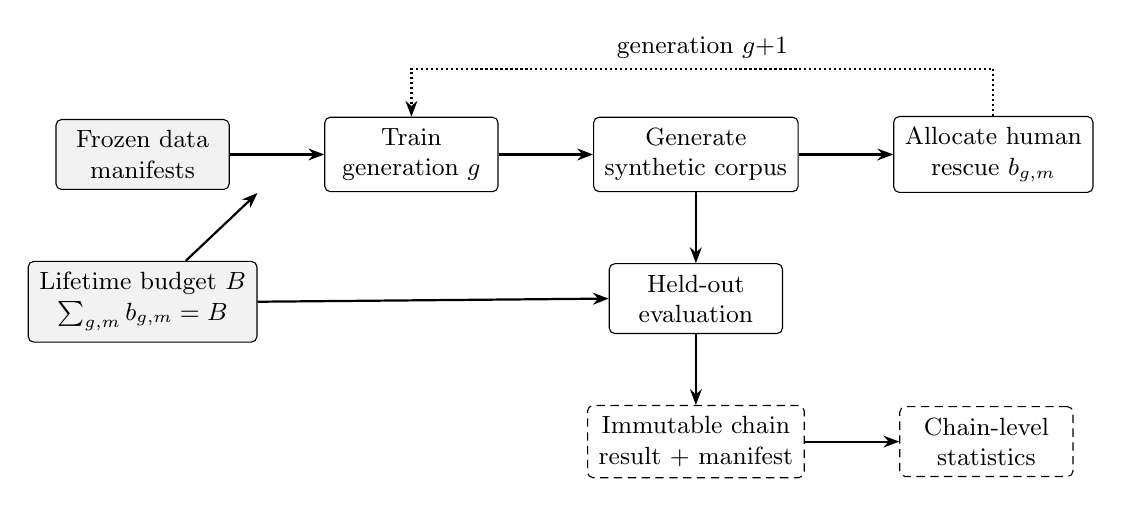
\begin{tikzpicture}[
  node distance=9mm and 12mm,
  every node/.style={font=\small},
  stage/.style={
    draw, rounded corners=2pt, align=center,
    minimum height=8mm, minimum width=22mm, inner sep=4pt
  },
  frozen/.style={stage, fill=black!5},
  artifact/.style={stage, densely dashed},
  flow/.style={-{Stealth[length=2mm]}, thick},
  feedback/.style={-{Stealth[length=2mm]}, thick, densely dotted},
]

  \node[frozen] (manifests) {Frozen data\\manifests};
  \node[stage, right=of manifests] (train) {Train\\generation $g$};
  \node[stage, right=of train] (generate) {Generate\\synthetic corpus};
  \node[stage, right=of generate] (allocate) {Allocate human\\rescue $b_{g,m}$};

  \node[frozen, below=of manifests] (budget) {Lifetime budget $B$\\$\sum_{g,m} b_{g,m} = B$};
  \node[stage, below=of generate] (evaluate) {Held-out\\evaluation};
  \node[artifact, below=of evaluate] (chain) {Immutable chain\\result + manifest};
  \node[artifact, right=of chain] (analysis) {Chain-level\\statistics};

  \draw[flow] (manifests) -- (train);
  \draw[flow] (train) -- (generate);
  \draw[flow] (generate) -- (allocate);

  % The recursion: this generation's allocation feeds the next generation's training.
  \draw[feedback] (allocate.north) -- ++(0,6mm) -| node[pos=0.25, above] {generation $g{+}1$} (train.north);

  \draw[flow] (budget) -- (allocate.south -| budget.east) ;
  \draw[flow] (budget.east) -- (evaluate.west);
  \draw[flow] (generate.south) -- (evaluate.north);
  \draw[flow] (evaluate) -- (chain);
  \draw[flow] (chain) -- (analysis);

\end{tikzpicture}

\caption{Recursive train--generate--allocate--evaluate pipeline. Shaded boxes are
frozen before any run. Dashed boxes are immutable artifacts. The dotted edge is
the recursion: generation $g$'s allocation enters generation $g{+}1$'s training
mixture. The lifetime budget constrains every allocation jointly, so spending
early reduces what remains for later generations.}
\label{fig:pipeline}
\end{figure}

\section{Data Appendix}
\label{app:data}

\textbf{RESULT\_PENDING.} The primary domain is not yet frozen
(\texttt{DECISIONS.md} U-002). This appendix records what will be reported once it
is, and is structured so that filling it requires no reorganisation.

\begin{itemize}
  \item Dataset identifier, revision hash, and licence, with the licence audit
    that selected it over the audited alternatives.
  \item Preprocessing: tokenizer identity and revision, normalisation, and the
    exact filter chain, each with a content hash.
  \item Partition statistics for all five partitions --- base training, rescue
    candidates, prompts, validation, and final test --- reporting example counts,
    token counts, and per-partition manifest hashes.
  \item The frozen mode definition, the number of modes $M$, and the criterion
    separating tail modes from common modes.
  \item Overlap report: exact and near-duplicate checks across every partition
    pair, with the near-duplicate threshold declared before it was applied.
\end{itemize}

Final test data influences no prompt, selection decision, threshold, stopping
rule, or hyperparameter. This constraint is enforced by the disjointness tests
rather than asserted.

\section{Evaluation Appendix}
\label{app:evaluation}

\textbf{RESULT\_PENDING.} The primary tail-retention definition is not yet frozen
(U-004). Two candidates are implemented and audited for determinism,
independence from the policy's selection signal, sensitivity to tail degradation,
discriminant validity against non-tail modes, and split-half reliability.

Held-out human negative log-likelihood is computed from target-token log
probabilities on the frozen test partition. Regret is aggregated across the
horizon as the area under the generation-wise curve.

Both tail candidates are computed without reference to the policy's
under-coverage score, so no policy can be rewarded for agreeing with its own
selection signal. This is a structural property of the interfaces, not a
convention.

\section{Statistics Appendix}
\label{app:statistics}

\textbf{RESULT\_PENDING.} Uncertainty is computed across independent chains.
Multiple generations within one chain are repeated observations and do not
increase the effective sample size.

The primary contrast is the joint policy against the strongest eligible non-joint
baseline, paired by chain seed. Paired differences are summarised by their mean
with a bootstrap interval resampled over complete chains. The smallest
scientifically meaningful effect is frozen before outcomes are opened (U-006),
and the interpretation that follows is selected mechanically from precommitted
templates covering favourable, null, harmful, and uncertain outcomes.

\section{Reproducibility Appendix}
\label{app:reproducibility}

Every value reported in this paper is generated by a script and traced to an
immutable artifact. No number is entered by hand.

\begin{itemize}
  \item \textbf{Positive control.} Upstream repository and exact commit are
    pinned before execution, together with the resolved framework versions and
    tokenizer revision actually used. Deviations from the upstream configuration
    are declared before running, never after observing a result.
  \item \textbf{Run artifacts.} Each chain emits a run manifest and a chain
    result validated against versioned JSON schemas. A three-state validator
    classifies each run as valid, valid with limitation, or invalid; blocking
    failures include budget-equality violations, identity mismatches, and
    impossible token accounting.
  \item \textbf{Budget matching.} Every policy in a comparison consumes identical
    lifetime human-origin optimizer tokens and identical total optimizer tokens.
    Equality is checked before launch from configuration and again after the run
    from emitted artifacts.
  \item \textbf{Token accounting.} Counts derive from tokenized batches actually
    consumed by the optimizer. Repeated presentation of an example costs its
    tokens once per presentation; gradient accumulation counts every micro-batch;
    resume neither double-counts nor drops the batch spanning a checkpoint.
  \item \textbf{Determinism.} Seeds propagate through sampling, generation,
    initialisation, dropout, and evaluation. Checkpoints carry content digests so
    silent corruption cannot survive a resume.
  \item \textbf{Generated outputs.} Tables and figures are emitted by scripts and
    recorded with SHA-256 digests in an artifact manifest, so a reader can verify
    that a figure is the one the pipeline produced.
\end{itemize}

\section{Limitations of Scope}
\label{app:scope}

\textbf{RESULT\_PENDING.} The planned study covers one licensed domain, one
124M--160M screening model, and one horizon. It cannot establish behaviour at
larger scales, in other domains, or for other model families. Any claim beyond
the tested configuration is future work and is marked as such.

\end{document}
